\chapter{Introduction \label{ch:Introduction}}

\section{Bulk metallic glasses: results from experiments}

\subsection{Bulk metallic glasses and the glass transition\label{sec:UndeformedGlasses}}

Several kinds of metallic glasses exist, differing by composition. Most of them are alloys of transition metals, such as Zr, Al, Ni and Cu. They are obtained by fast cooling (quenching) a hot melt composed by such elements fast enough so to avoid crystallization, so that atoms do not arrange themselves in ordered lattices. If the choice of the elements and their concentration is such that crystallization does not occur, the mixture is said to have ``good glass forming capabilities''. If bulk solid samples can be obtained, the result is a \emph{bulk metallic glass}. There is no set of precise rules to determine if a given melt will be a good glass former, but still some features have been shown to be beneficial to impede crystallization \cite{chen2011brief, inoue2000stabilization}:
\begin{itemize}
	\item consituting elements should have negative heat of mixing, so that unlike elements stick together forming energetically favored structures, rather than separating into pure phases;
	\item elements should have different sizes. Size is seen to play a major role in determining whether crystal structures are favored over disordered ones;
	\item mixtures should be contain more than three elements. Intuitively, the rationale behind this requirement is to make crystal configurations more complex and harder to reach in configuration space. However (as in the Duwez experiment \cite{klement1960noncrystalline}), binary mixtures also show glass forming capabilities. 
\end{itemize}
As for the choice of the composition, eutectics are, generally speaking, better glass formers. In multicomponent systems, however, eutectic points are hard to find because of the complexity of the phase diagrams. An additional difficulty is represented by the fact that the best glass  formers have a narrow compositional range.\\
If the criteria above are satisfied, the melt can avoid crystallization as temperature is lowered, and enter in a \emph{supercooled state}. At a microscopic level, supercooled configurations are very similar to those assumed in the liquid state, and thus characterized by absence of long range order. In such a state, the shear viscosity $\eta$ is seen to dramatically increase with decreasing temperature (see for example \cite{bakke1995viscosity}), and experimental data on the shear viscosity can be fit by the Vogel-Fulcher-Tammann law:
\begin{equation}
	\eta = \eta_{0}\, e^{\frac{B T_{0}}{T-T_{0}}}
	\label{eq:VogelFulcher}
\end{equation}
where $\eta_{0}$ and $B$ are constants. 
The consequence of \autoref{eq:VogelFulcher} is that at some temperature $T_{g}$ (named the \emph{glass transition temperature} \cite{ediger1996supercooled}) well above $T_{0}$ the viscosity becomes so high that samples behave like solids on experimental timescales, and as such can sustain shear stress, even though the microscopic structure is disordered and similar to that of liquids. In that case, one says that a \emph{glass} has been formed. Incidentally the $T_{g}$ of metallic glasses is typically above room temperature, so that they are solid in ambient conditions. 
Data on $\eta$ for several bulk metallic glass formers and other systems are plotted in \autoref{fig:BMGAngellPlot} as a function of the inverse temperature, rescaled by the respective $T_{g}$ (see also \cite{ediger1996supercooled}). 
\begin{figure} 
\centering 
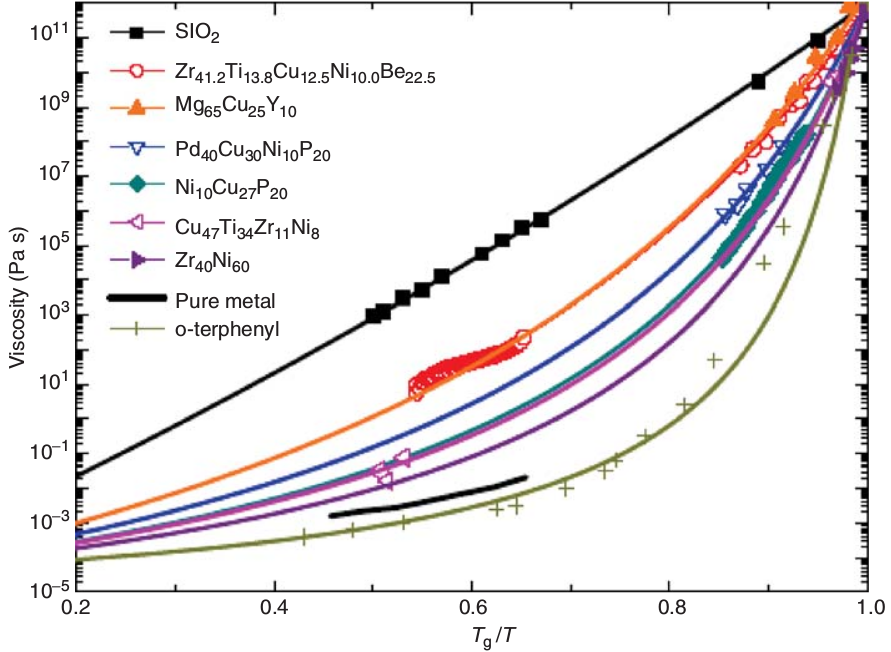
\includegraphics[width=0.8\textwidth]{BMGAngellPlot.png} 
\caption{Plot of the viscosity as a function of the normalized inverse temperature $T_{g}/T$ for different metallic glass formers in their supercooled state. Such a plot is often called ``Angell plot'' in the literature \cite{debenedetti2001supercooled}. $T_{g}$ is defined as the temperature at which a given system as a viscosity of $10^{12}$ Pa s. Fits using \autoref{eq:VogelFulcher} are superimposed. For reference, data relative to ortho-terphenyl and SiO$_{2}$ are reported. Metallic glass formers show a behavior which is qualitatively similar to that of ortho-terphenyl, and thus are classified as \emph{fragile} glass formers (see text). From \cite{busch2007thermodynamics}. \label{fig:BMGAngellPlot}}
\end{figure}
Metallic glasses in this plot show a non-exponential dependence from $T_{g}/T$, and thus belong to the class of \emph{kinetically fragile} glass formers (as ortho-terphenyl), differing from the so-called \emph{kinetically strong} ones (such as SiO$_{2}$), which instead show an exponential dependence of $\eta$ on the inverse temperature. \\
The temperature $T_{g}$ marks not only the transition from a (supercooled) liquid to a solid-like state, but also the passage from an equilibrium state (metastable with respect to crystallization) to a regime where the sample appears to be \emph{out of thermodynamical equilibrium}. The absence of equilibrium below $T_{g}$ translates into a very slow drift of mechanical, calorimetric and electrical properties \cite{luo2006aging, khonik2012comparative} with time and their dependence on the detailed thermal history of the sample during the quench. In fact, the material behaves differently depending on its \emph{age}, i.e. the time elapsed since the cooling of the sample below $T_{g}$. This phenomenon of \emph{aging} is accompanied by an evolution of the structure at the microscopic level (also called \emph{structural relaxation}), and can be measured in metallic glasses via X-ray photon correlation spectroscopy \cite{ruta2012atomic} or positron annihilation lifetime spectroscopy \cite{wang2005ageing}. \\
Another phenomenon that is observed in metallic glass melts below $\approx 1.2\, T_{g}$ is the breakdown of the Stokes-Einstein relation \cite{chathoth2010stokes}, which states that
\begin{equation}
	\frac{D\eta}{T} = c
	\label{eq:StokesEinstein}
\end{equation}
where $D$ is the translational diffusion coefficient and $c$ is a constant.

\subsection{Mechanical properties of metallic glasses \label{sec:DeformedGlasses}}

Below $T_{g}$ bulk metallic glasses exhibit remarkable mechanical properties. In tensile deformation experiments (see \autoref{app:Glossary} for a glossary of terms relative to the properties of materials subjected to tensile experiments), they behave elastically (so that stress deviates very little from a linear function of strain) up to high values of strain. In fact the yield strain is $\approx 0.02$, which is close to that of polymeric materials and an order of magnitude larger than the value $\approx 0.002$ of typical crystalline metals. This fact, combined with Young moduli comparable to those of crystalline metals, allows them to exhibit very high \emph{strengths} (see \autoref{fig:BMGStrength}). 
The high yield strain and the high values of the Young modulus make it possible to store elastically in bulk metallic glasses large quantities of energy per unit volume, endowing them with high values of \emph{resilience} (see \autoref{fig:BMGStorage}). Furthermore, their \emph{loss coefficient} is extraordinarily low. 
All the properties listed above are in general desirable for applications: strength allows to sustain large loads without undergoing irreversible deformation, enhancing durability; high strength incidentally translates into high \emph{hardness}, which means resistance to wear;
high resilience and low energy losses make bulk metallic excellent candidates for spring applications, where mechanical energy needs to be stored and recovered.

\begin{figure} 
\centering 
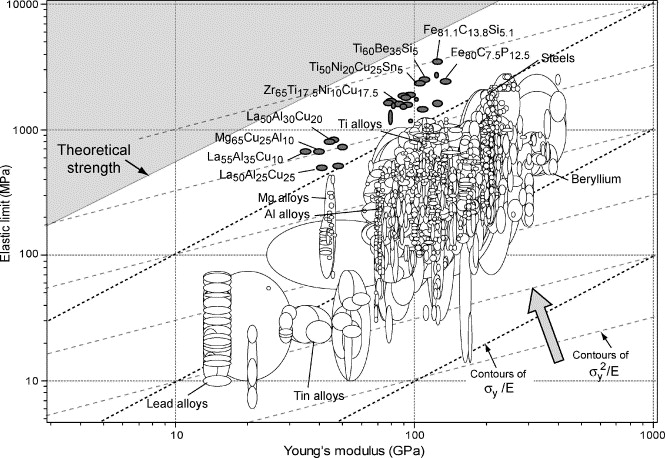
\includegraphics[width=0.9\textwidth]{BMGStrength.jpg} 
\caption{Strength (here named ``elastic limit'') and Young modulus for various materials. This kind of plot, with two material properties on the axes and ellipses enclosing the values relative to different materials, is called in the literature ``Ashby plot'' \cite{ashby2005materials}. Data relative to metallic glasses are enclosed by darker ellipses. Thanks to their exceptional strength, metallic glasses lie well above materials with a comparable Young modulus. From \cite{ashby2006metallic}. \label{fig:BMGStrength}}
\end{figure}

\begin{figure} 
\centering 
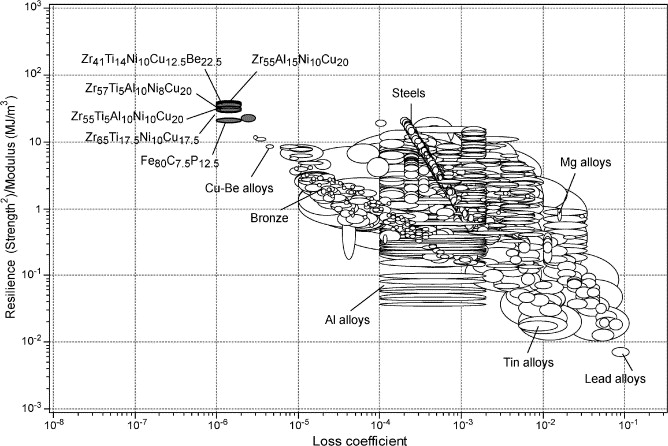
\includegraphics[width=0.9\textwidth]{BMGLossResilience.jpg} 
\caption{Ashby plot of the resilience and loss coefficient for various materials. Metallic glasses are outliers, as they can store very high amount of energy per unit volume (high resilience) and dissipate very low amounts of the stored energy when they undergo cyclic deformation (low loss coefficient). From \cite{ashby2006metallic}. \label{fig:BMGStorage}}
\end{figure}

However, metallic glasses possess some characteristics that limit their widespread adoption in applications. Notably, if a sample made of metallic glass is deformed beyond its yield strain it typically exerts lower and lower forces. In fact, contrary to what is commonly observed in crystalline metals, metallic glasses undergo work \emph{softening} upon loading. For strains slightly above the elastic limit deformation becomes localized in \emph{shear bands} and leads to catastrophic failure (see \autoref{fig:BMGBrittleFailure}). For this reason, metallic glasses are said to be \emph{brittle}, and are not as \emph{ductile} as metals that are able to undergo large \emph{plastic} deformations beyond their elastic limit. This is clearly a drawback in structural applications, where one would like a material to be able to sustain large strains before rupturing.
Another drawback is the low fatigue limit \cite{schuh2007mechanical} observed for some metallic glasses. When deformed cyclically, metallic glasses can exhibit fatigue cracks even well below their yield strain \cite{peter2002fatigue}. This also limits their reliability under cyclic loads.

\begin{figure} 
\centering 
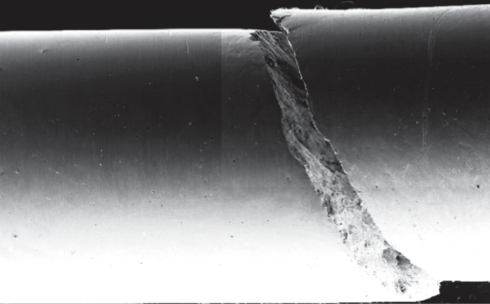
\includegraphics[width=0.6\textwidth]{BMGBrittleFailure.jpg} 
\caption{Tipical brittle fracture of a metallic glass rod subjected to tensile strain. Metallic glasses don't typically show the necking behavior shown by ductile metals. Adapted from \cite{hofmann2008designing}. \label{fig:BMGBrittleFailure}}
\end{figure}

\subsubsection{Rejuvenation and overaging}
A debated issue in the context of deformed glasses is the possibility to revert the state of an aged (in the sense of \autoref{sec:UndeformedGlasses}) glassy sample to a state where it shows properties that it had at an earlier stage of the aging process. This phenomenon goes under the name of \emph{rejuvenation} and has been observed in calorimetric experiments on metallic glasses \cite{concustell2009structural}. \\ 
As mentioned above in the context of fatigue, oscillatory load can lead to changes in the material. In some cases \cite{packard2008hardening} cyclic deformation makes the properties of samples similar to those that one would expect to find in \emph{more aged} samples. In these cases, when mechanical deformation is seen to accelerate the process of aging, one speaks of \emph{overaging}.

\section{Theoretical models and computer simulations}

The impressive increase in viscosity, the phenomenon of \emph{aging} and the breakdown of the Stokes-Einstein relation are shared by other \emph{glass forming} materials, and have been problems that have puzzled physicists for a very long time. An introduction to these and other aspects of the glass transition is given in \cite{cavagna2009supercooled} and in several other recent reviews on the subject (\cite{binder2011glassy, berthier2011theoretical, ediger2012perspective} just to name a few).\\
Here we present one of the most important frameworks used in the literature of the physics of glasses to rationalize their behavior, namely that of 
potential energy landscape (PEL) \cite{sciortino2005potential, heuer2008exploring}, which will be extensively used throughout this thesis. 

\subsection{The Potential Energy Landscape}

\subsubsection{Geometrical properties of the energy landscape}
Here we want to describe a supercooled liquid, or a glass, at a fine-grained level, that is by decomposing it into the set of interacting atoms\footnote{The same approach can be applied to molecular, or colloidal glasses as well. In that case however the simplest element won't be an atom, but an entire molecule (as in the case of a \emph{molecular glass}) or a colloidal particle \emph{in the case of a colloidal glass}, with its degrees of freedom.} that form it. Each of the $N$ atoms in a given system is thus thought to have (in 3 dimensions) 6 translational degrees of freedom, which evolve according to a set of Hamilton's equations of motion in a volume $V$. The potential part of the Hamiltonian takes into account the nuclear and electronic degrees of freedom in a coarse grained way, ``condensing'' them in the $6N$ spatial coordinates and velocities of the nuclei. In particular, the potential energy function $U$ can be expressed as a function of the coordinates of the nuclei:
\begin{equation}
	U(\mathbf{r_{1}, \ldots, r_{N}})
	\label{eq:TotalPotentialEnergy}
\end{equation}
where $\mathbf{r_{i}}$ is the position of the $i$-th atom. 
In this view, the system can be represented as a point moving on the $3N + 1$-dimensional surface $(\mathbf{r_{1}, \ldots, r_{N}}, U(\mathbf{r_{1}, \ldots, r_{N}}))$. Such surface is named in the literature ``potential energy landscape'' (PEL) and is characterized by ``peaks'' (in correspondence of configurations with a large potential energy with respect to neighboring configurations), ``valleys'' (energetically favored configurations) and ``mountain passes'' separating different valleys.\\
It is useful to note that any external perturbation $\Delta U$ dependent on the coordinates of the particles of the system changes the form of the energy landscape:
\begin{equation}
	U'(\mathbf{r_{1}, \ldots, r_{N}}) = U(\mathbf{r_{1}, \ldots, r_{N}}) + \Delta U(\mathbf{r_{1}, \ldots, r_{N}})
	\label{eq:PerturbedTotalPotentialEnergy}
\end{equation}
We will describe in detail in \autoref{ch:ParticleModels} how an externally imposed mechanical deformation acts like such a perturbation, and this fact will be of fundamental importance in our analysis.

Important points of the potential energy landscape are its local minima. In a local potential energy minimum the system is mechanically stable: the force on each particle is zero and imposing a small displacement on one of them originates a force that tends to put it back in its original position, in a way that depends on the Hessian of the potential at the minimum. Incidentally, any configuration can be mapped onto one of such energy minima\footnote{Strictly speaking this is not \emph{always} true: if the steepest descent algorithm is used, for instance, critical points as local maxima and saddle points (and points mapping to saddles through steepest descent) can't be unambiguously associated to a local minimum. Such points, however, are expected to belong to a measure zero set anyway.} once that a energy minimization procedure is adopted. Such minima are called \emph{inherent structures} or \emph{inherent configurations} \cite{stillinger1995topographic}. Note that once that a minimization strategy is set, the configuration space is partitioned into different \emph{basins}, each basin being formed by the points mapping onto the same inherent structure through the minimization procedure.\\
The energy landscape is a surface in a highly dimensional space, and as such it is hard to have an intuitive understanding of it and of its inherent structures. A better intuition of some of its features can be obtained by means of a simple argument and a graphical representation.
The simple argument leads to the conclusion that \emph{the number of inherent structures is exponential in the number of particles $N$}. To understand this, consider a system composed of a large number of particles $N$, and divide it into $L$ subsystems composed by $n$ particles. If $n$ is sufficiently large, and the potential between the particles is short ranged, one can safely assume that the influence of each subsystem on the other subsystems is weak, and treat them as independent. If the subsystems are independent, the supersystem is in an inherent structure if and only if each of its subsystems is in an inherent structure. If we call the number of inherent structures of each subsystem $m$, the number of inherent structures $M$ is given by 
\begin{equation}
	M = m^{L} = m^{N/n}
\end{equation}
The consequence of this fact is that the landscape becomes very complex as $N$ increases, and a detailed enumeration of the local minima of the landscape becomes unfeasible for systems composed by more than a few dozen of particles \cite{doye1999evolution}. \\
The useful way to represent energy landscapes mentioned above consists in drawing \emph{disconnectivity graphs} \cite{becker1997topology}. 
To construct a disconnectivity graph for a given potential energy landscape one initially picks a low threshold value of the energy. At that value of the threshold, some pockets of the configuration space will contain configurations whose energy is lower than the threshold. As the energy threshold is increased, some pockets coalesce, and others will appear (see \autoref{fig:LandscapePocketsCoalescence} for an example with an energy landscape in two dimensions\footnote{Refer to \cite{becker1997topology} for plenty of one-dimensional examples.}). A disconnectivity graph encodes the information about how many disconnected pockets exist at a given energy and at what energy coalescences between them occur. The disconnectivity graph relative to the landscape in \autoref{fig:LandscapePocketsCoalescence} is given in \autoref{fig:DisconnectivityGraph}.\\
Using terminology of graph theory \cite{bollobas1998modern}, a disconnectivity graph is a \emph{tree} and each of its \emph{leaves} is associated to an inherent structure, whereas the \emph{internal vertices} are associated to barriers in the landscape.
\begin{figure} 
\centering 
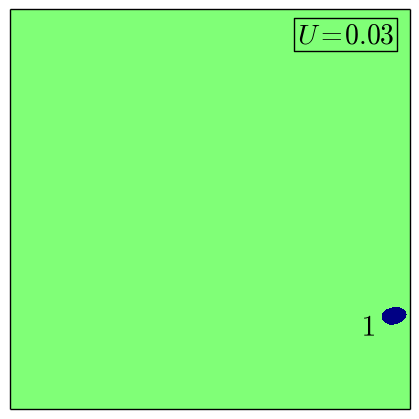
\includegraphics[width=0.32\textwidth]{landscape-1.png} 
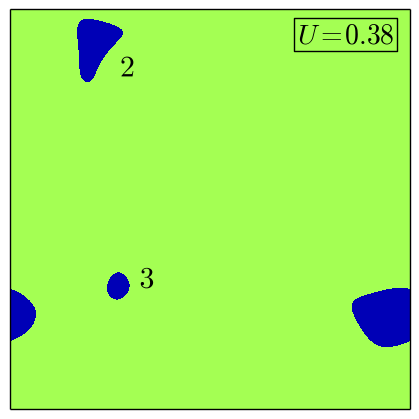
\includegraphics[width=0.32\textwidth]{landscape-2.png} 
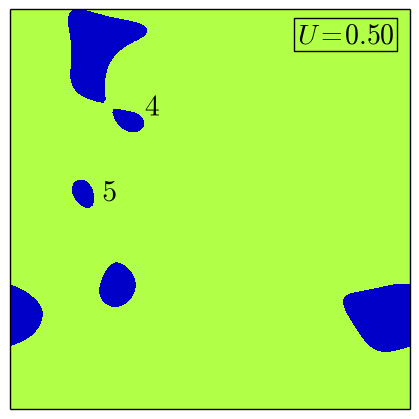
\includegraphics[width=0.32\textwidth]{landscape-3.png} \\
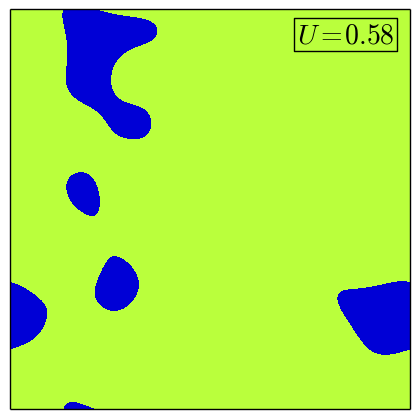
\includegraphics[width=0.32\textwidth]{landscape-4.png} 
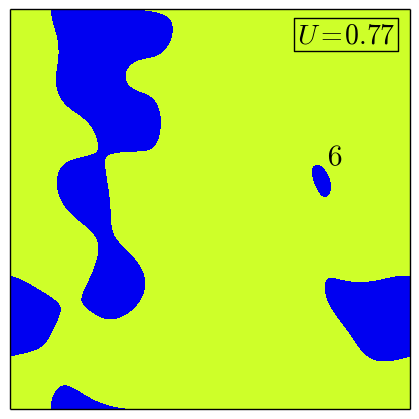
\includegraphics[width=0.32\textwidth]{landscape-5.png} 
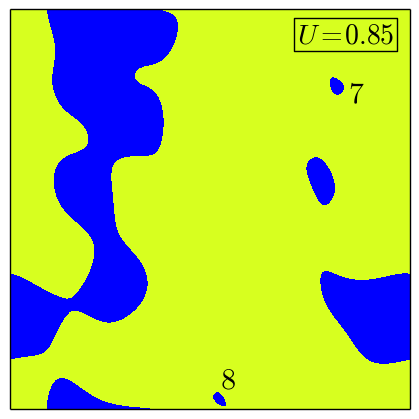
\includegraphics[width=0.32\textwidth]{landscape-6.png} 
\caption{Schematic representation in 2D of an energy landscape. Regions of the energy landscape in \autoref{fig:FullLandscape} that lie below and above the threshold value specified in the legend. Pockets with energy lower than the threshold value are drawn in blue. These are labeled so to be associated to the disconnectivity graph in \autoref{fig:DisconnectivityGraph}. \label{fig:LandscapePocketsCoalescence}}
\end{figure}
\begin{figure} 
\centering
\begin{subfigure}[b]{0.55\textwidth}
	\centering
	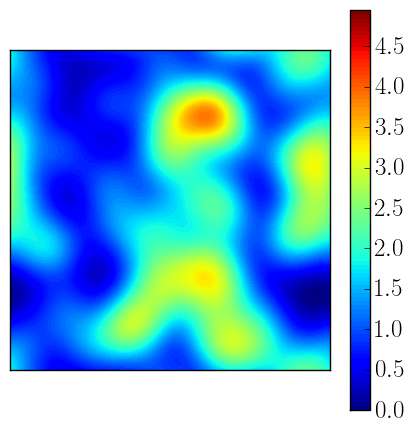
\includegraphics[scale=0.5]{landscape.png}
	\caption{\label{fig:FullLandscape}}
\end{subfigure}
\centering
\begin{subfigure}[b]{0.4\textwidth}
	\centering
	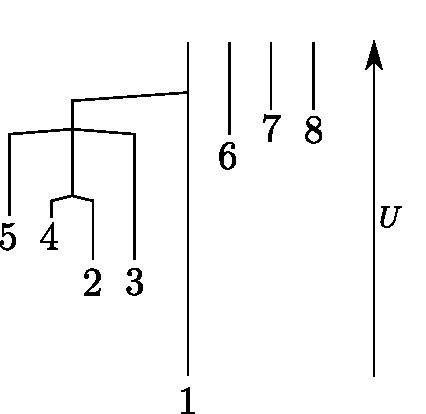
\includegraphics[scale=0.5]{Disconnectivity.pdf} 
	\caption{\label{fig:DisconnectivityGraph}}
\end{subfigure} 
\caption{(\subref{fig:FullLandscape}) Schematic representation in 2D of an energy landscape, which is supposed here to have only two degrees of freedom. The heat map describes the potential energy of the landscape used in \autoref{fig:LandscapePocketsCoalescence}. (\subref{fig:DisconnectivityGraph}) Disconnectivity graph of the deepest minima of \autoref{fig:FullLandscape}.}
\end{figure}
An example of a (part of a) disconnectivity graph for a system of Lennard-Jones particles (taken from \cite{desouza2009connectivity}) is given in \autoref{fig:LJDisconnectivityGraph}.

\begin{figure} 
\centering 
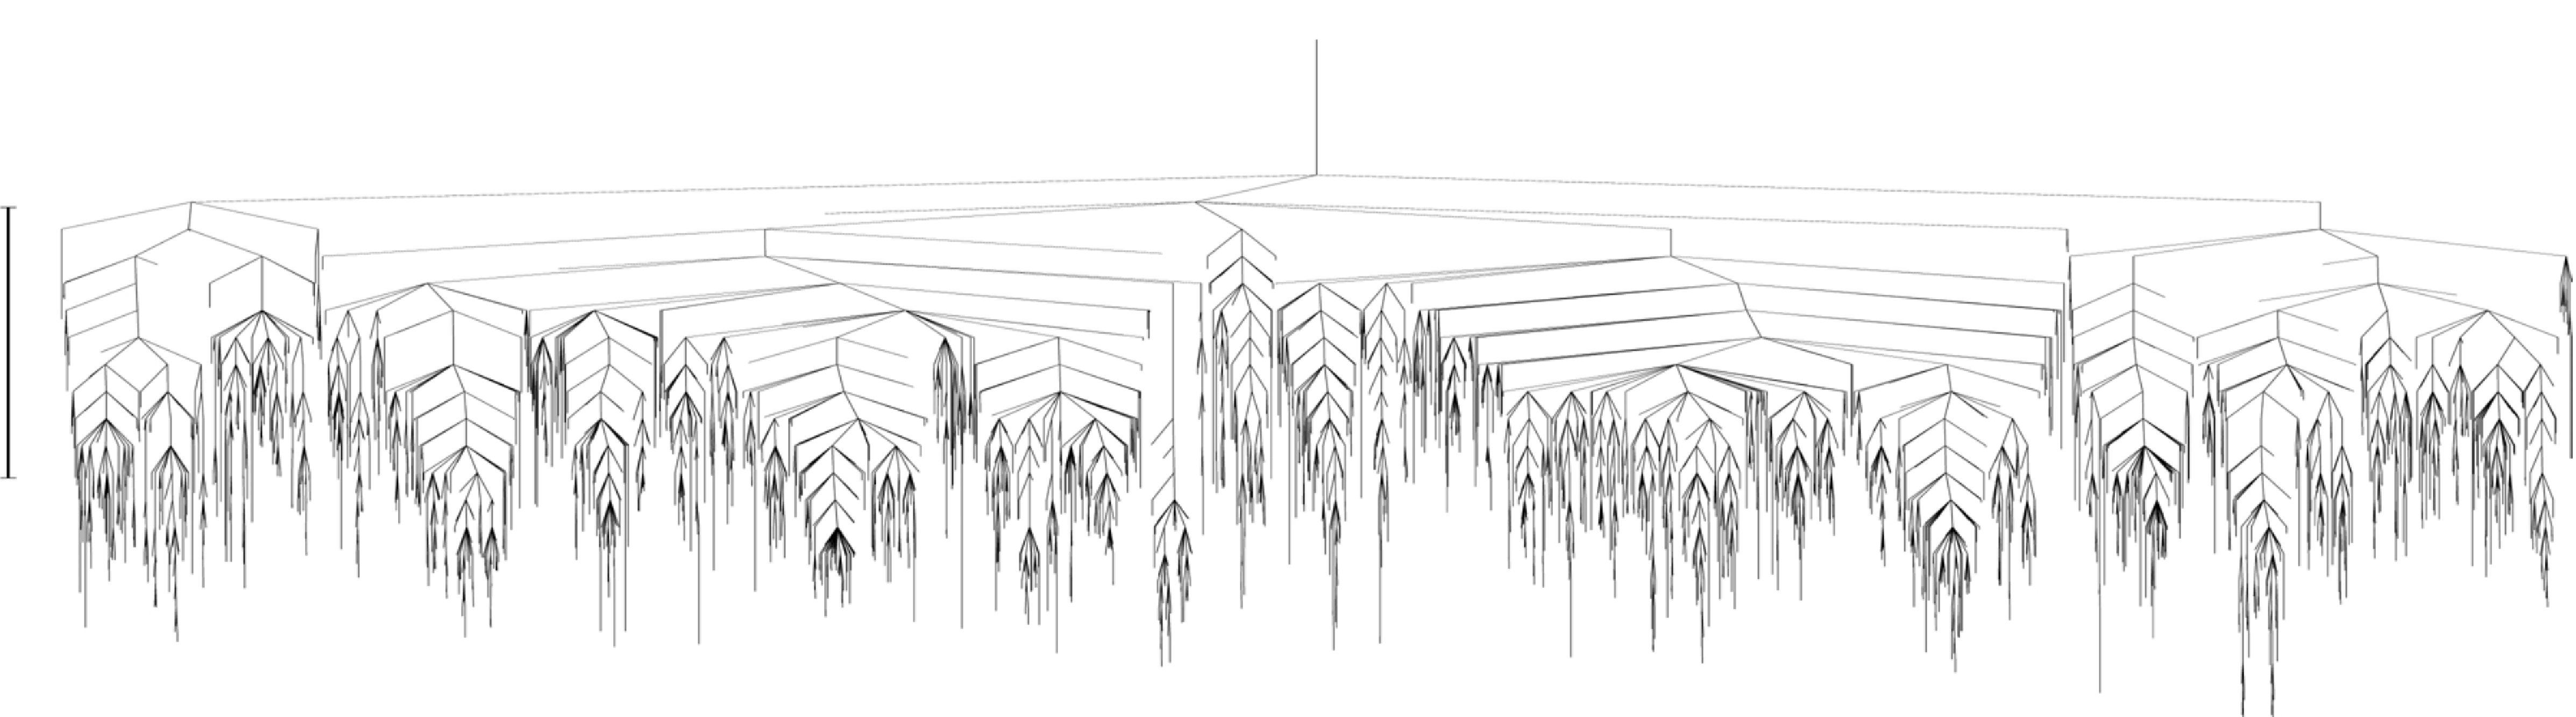
\includegraphics[width=\textwidth]{LandscapeLJ.png} 
\caption{Disconnectivity graph for a Lennard-Jones binary mixture. Adapted from \cite{desouza2009connectivity}. \label{fig:LJDisconnectivityGraph}}
\end{figure}

\subsubsection{Dynamics in the energy landscape}

The idea behind the landscape approach is that the way the system evolves in configuration space is affected by the topography of the landscape. 
At high temperature, the system has a total energy large enough to be able to visit different configurations with probabilities that are only slightly influenced by the value of the potential energy of such configurations. This is because the probability density is proportional to the Boltzmann factor $e^{-\beta U(\mathbf{r_{1}, \ldots, r_{N}})}$  (where $\beta$ is $1/k_{B} T$). If the temperature is high enough, one can consider that for the majority of configurations $U \ll kT$ so that their probability density is almost constant. In this regime the system is able to overcome the barriers that separate different basins, and the motion of the system is not affected much by the landscape. Note that as the system doesn't visit preferentially any part of the landscape, the average properties of the configurations that the system visits are simply related to the volume of configuration space associated to them\footnote{This is a simple consequence of the fact that the average value of an observable $A$ that depends only on the positional degrees of freedom is $\langle A \rangle = \int A(\mathbf{R}) e^{-\beta U(\mathbf{R})} d\mathbf{R}$, and this expression, in the case of high $T$, simplifies in $\langle A \rangle = \int A(\mathbf{R}) d\mathbf{R}$.}.\\
At lower temperature the system explores preferentially low potential energy regions of the landscape, and has difficulties in crossing the potential energy barriers in the landscape. In this case the landscape is able to confine the system for some time within some of its basins, thus slowing down its dynamics and reducing its ability to relax stress fluctuations. This fact is at the root of the viscosity behavior described by \autoref{eq:VogelFulcher}.
The details of the microscopic dynamics have been related to the features of the depth and topology of the landscape \cite{doliwa2003hopping}, and the landscape approach has proved successful in predicting quantitatively the behavior in \autoref{eq:VogelFulcher} \cite{sastry2001relationship} and rationalize the phenomenon of aging \cite{mossa2004crossover}. 

The dynamics of systems in the landscape can be studied using numerical simulation techniques like Molecular Dynamics (MD). In MD $N$ particles (in our case representing atoms in a solid) are let evolve according to their interaction potential $U$ in \autoref{eq:TotalPotentialEnergy} in a way that mimics their dynamics in real materials. In a simulation, particle positions are known at any point in time, an information that is experimentally inaccessible in the case of atoms in the bulk of real materials. This means that computer simulation allows to \emph{track the motion of systems in their energy landscape} and gather microscopic insight about their macroscopic behavior \cite{heuer2008exploring}.\\
In the case of metallic glasses, constituent atoms can be simulated as point particles interacting via a so-called embedded atom potential (or EAM potential) \cite{daw1993embedded}. Potentials of this class can be written in the form
\begin{equation}
U = \sum_{i=1}^{N} \sum_{j<i} \phi(|\mathbf{r_{i} - r_{j}}|) + \sum_{i = 1}^{N} F(\rho_{i}(\mathbf{r_{i}})) \qquad \rho_{i}(\mathbf{r_{i}}) = \sum_{\substack{j = 1\\ j \neq i}}^{N} \psi (|\mathbf{r_{i} - r_{j}}|)
\label{eq:EAMpotential}
\end{equation}
where $\phi$ is a pair potential interaction, $\psi$ represents the electron density around a nucleus, and $F$ is the so-called \emph{embedding function}. The function $\rho_{i}$, according to its definition, can be thought as the sum of the electronic densities due to all the atoms but the one labeled with $i$. If $F$ was linear in $\rho$, \autoref{eq:EAMpotential} would reduce to a simple pairwise additive potential. In the embedded atom method, however, $F$ is non-linear, so that \autoref{eq:EAMpotential} is a many-body potential, which takes into account the fact that the presence of an atom alters the strength of the interaction between the other atoms. The detailed functional forms of $F$, $\rho$, $\phi$ and $\psi$ can be determined from first principles using ab-initio methods \cite{daw1993embedded}.\\
An accurate, quantitative description of a material can be traded for simplicity by using a simple pairwise additive potential. This choice is often done in the literature whenever one is more interested in a qualitative, general description of a phenomenon rather than in the determination of the behavior of a specific material. A popular choice in this sense is represented by the Lennard-Jones (LJ) potential:
\begin{equation}
U = \sum_{i=1}^{N} \sum_{j<i} \phi(|\mathbf{r_{i} - r_{j}}|) \qquad \phi(r) = 4\epsilon \left[\left(\frac{\sigma}{r}\right)^{12} - \left(\frac{\sigma}{r}\right)^{6}\right]
\label{eq:LennardJonesPotential}
\end{equation}
which describes accurately the interaction between noble gases such as Ar, Kr, Xe, but has also been employed (in its multi-component generalization) to model mixtures of Ni and P \cite{kob1995testing}. 

\subsection{Results from simulations of glasses relevant for this work \label{sec:PreviousWorkOnOveragingAndRejuvenation}}
The analysis of the trajectories of particles interacting with potentials like those in \autoref{eq:EAMpotential} and \autoref{eq:LennardJonesPotential} in dense systems has revealed features of their motion such as \emph{dynamic heterogeneities} and an increasing \emph{cooperativity} in particle motion as $T$ is lowered in the supercooled and glassy states. These observations have been successively confirmed by experiment \cite{berthier2005direct}. The possibility to measure accurately the structure has also allowed the search of \emph{structural} signatures of glassy behavior, and growing \emph{static} lengthscales (i.e. not related to dynamics, but to the mere arrangement of the particles at a given time) at the root of the viscosity behavior in \autoref{eq:VogelFulcher} \cite{berthier2011theoretical}. \\
Rather than exploring the features listed above, which are related to the way \emph{undeformed} glasses behave, in this thesis we focus our attention on the behavior of glasses under deformation. 
Several techniques can be used to model the behavior of solids under deformation, and these in turn can be classified by their granularity, which is the resolution that they have in space and time. Such methods are extensively reviewed in \cite{rodney2011modeling} (with many more details than those mentioned here), where the possibility of combining them in a \emph{multiscale} approach is also discussed.
In this thesis, we try to understand what is the effect of \emph{cyclic shear deformation} on glassy samples at a \emph{microscopic} level, using techniques that are described in \autoref{ch:ParticleModels} and analyzed more extensively in \cite{rodney2011modeling} and \cite{falk2010simulating}. 
This is expected to give us insights about the phenomena seen in experiments where a sample is subject to a cyclic load, and to clarify the origin of mechanical \emph{rejuvenation} and \emph{overaging} mentioned in \autoref{sec:DeformedGlasses}.
Before doing so, we introduce here some results obtained in the past by means of simulation of Lennard-Jones systems. Such results are propedeutical in the understanding of the following chapters and lie at the foundations of the present work.

\subsubsection{Average $U$ of glasses obtained by cooling from finite $T$ to $0$ at infinite rate}
As we stated above, at low temperature a system is expected to assume configurations whose potential energy is low.
In \cite{lacks2004energy}, configurations of a binary mixture of Lennard-Jones particles equilibrated at temperature $T$ are quenched via an energy minimization procedure so to obtain the inherent structures to which they are associated. Physically, this operation corresponds to cooling the initial configuration to zero temperature at an extremely fast rate.
The value of the temperature of the equilibrated samples from which inherent structures are obtained via energy minimization is called \emph{effective temperature} of the corresponding inherent structures.
If one plots the average potential energy $U$ of such inherent structures as a function of their effective temperature, one gets a plot like that in \autoref{fig:UvsT}.
\begin{figure} 
\centering 
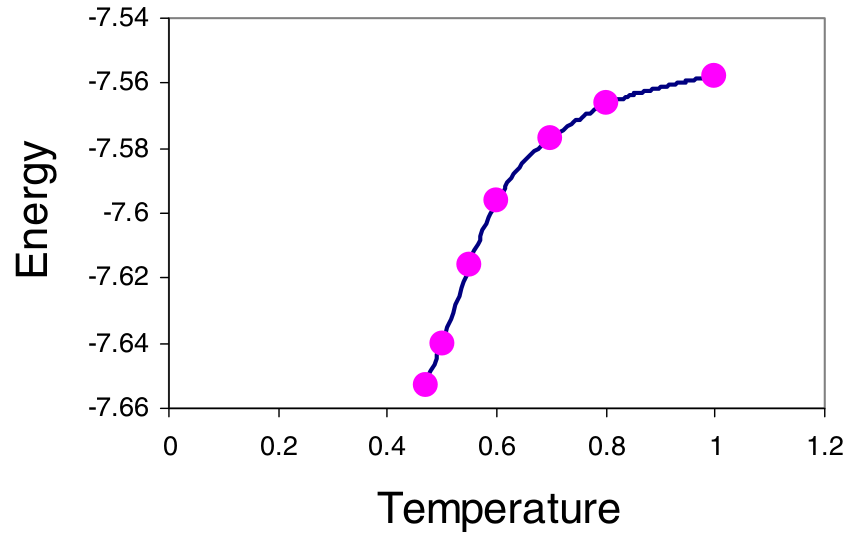
\includegraphics[width=0.7\textwidth]{UvsT.png} 
\caption{Average energy per particle for inherent configurations of a binary Lennard-Jones mixture obtained by quenching samples equilibrated at different $T$ at infinite rate. At low temperatures the quench brings the system to minima with average lower energy. From \cite{lacks2004energy}. \label{fig:UvsT}}
\end{figure}
At high $T$ the system can be thought as residing in a given energy basin for a time that depends more on the extent of the basin in configuration space rather than its depth\footnote{This is because the Boltzmann factor at high temperatures will be $\approx 1$ wherever the potential has a small absolute value, and this includes all states with a negative potential energy.}. Increasing $T$ further thus does not change the average energy after a quench (see \autoref{fig:UvsT}). At low temperatures the system will instead sample preferentially states with low energy, and thus spend time in deeper basins of the landscape. It's easy to believe that if the energy is minimized, the system will on average reach deeper inherent structures when starting from configurations equilibrated at lower $T$.
In the language of disconnectivity graphs, this means that at low $T$ the system spends more time in the basins associated to the leaves with the lowest energy in graphs like that in \autoref{fig:LJDisconnectivityGraph}.

\subsubsection{Average $U$ of glasses obtained by cooling from finite $T$ to $0$ at finite rates}
In \cite{utz2000atomistic}, a binary mixture of Lennard-Jones particles equilibrated at temperature $T$ is quenched to some lower temperature $T_{0}<T_{g}$ at a finite rate. As schematized in \autoref{fig:Aging}, faster cooling rates bring, at the end of the quench, to configurations of higher potential energy, whereas slower rates are more efficient in bringing the system in regions of the landscape with lower energy. Incidentally, samples quenched infinitely fast from equilibrium states at low $T$ in \cite{lacks2004energy} can be associated to the glassy states obtained by slow cooling in \cite{utz2000atomistic}, and a similar relationship exists between the states quenched infinitely fast from high $T$ and those which undergo fast cooling in \cite{utz2000atomistic}. In this way the results in \cite{utz2000atomistic} and \cite{lacks2004energy} can be compared.

\begin{figure} 
	\centering
	\begin{subfigure}[b]{0.45\textwidth}
		\centering
		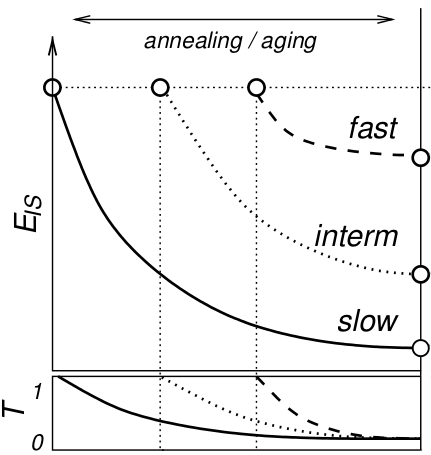
\includegraphics[scale=0.35]{Aging.png} 
		\caption{\label{fig:Aging}}
	\end{subfigure}
	\centering
	\begin{subfigure}[b]{0.45\textwidth}
		\centering
		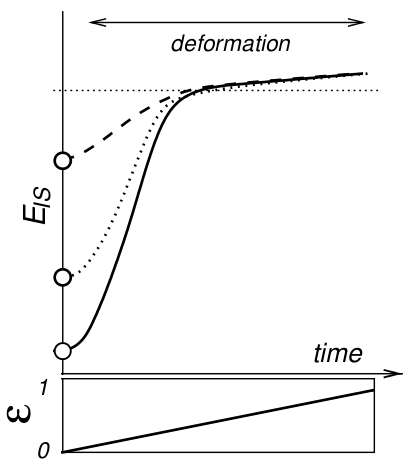
\includegraphics[scale=0.35]{Rejuvenation.png} 
		\caption{\label{fig:Rejuvenation}}
	\end{subfigure} 
\caption{(\subref{fig:Aging}) Qualitative behavior of the energy per particle (here called $E_{IS}$) as a function of time obtained by lowering the temperature at different rates (the $T$) and mapping the system onto its associated inherent structure. The lower panel shows the form of $T$ in time. The slowest quench yields the lowest final energies. (\subref{fig:Rejuvenation}) Energy per particle as a function of strain (here called $\epsilon$) obtained starting from the samples quenched at different shear rates in (\subref{fig:Aging}) and increasing the value of shear strain. From \cite{utz2000atomistic}.}
\end{figure}

\subsubsection{Effect on $U$ of deformation of glasses obtained by cooling at finite rates}

After having obtained glassy samples at $T_{0}$ with different cooling rates, authors in \cite{utz2000atomistic} shear their samples at zero temperature, with a protocol that will be described in detail in \autoref{ch:ParticleModels}. The potential energy of their samples increases with increasing strain $\gamma$, so that samples visit states whose energies are equal to those that they had in earlier and earlier stages of the aging process. The authors thus observe that, at least by judging from the value of the potential energy, samples seem to undergo \emph{rejuvenation} under deformation.

\subsubsection{Effect on $U$ of cyclic deformation of glasses obtained by cooling at infinite rates}

In \cite{lacks2004energy}, authors perform deformation of samples as zero temperature similar to those in \cite{utz2000atomistic}. Differently from \cite{utz2000atomistic}, the initial states are obtained by quenching at an \emph{infinite rate} samples equilibrated at different temperatures $T$.
In addition, rather than performing a simple shear deformation with monotonically increasing strain, authors in \cite{lacks2004energy} perform a single semicycle of shear deformation, where the strain is incremented from 0 to $\gamma_{max}$ and then decreased back to 0. In their case, again, the average potential energy of their samples is also seen to change with the deformation, and at the end of the semicycle the energy is observed to be higher or lower than the initial one (see \autoref{fig:OscillatoryRejuvenationLJ}).
\begin{figure} 
\centering 
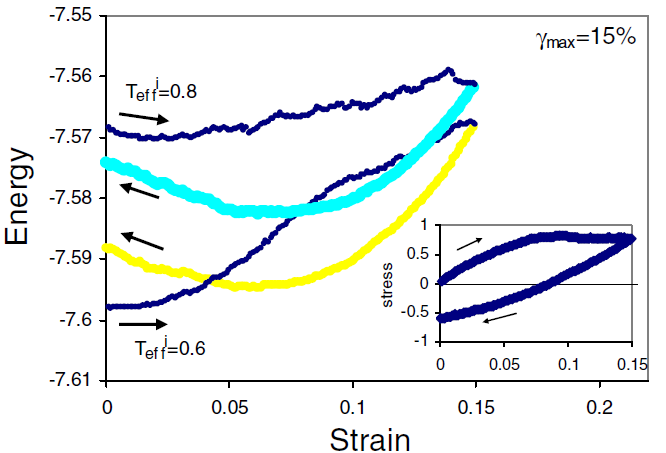
\includegraphics[width=0.7\textwidth]{OscillatoryRejuvenationLJ.png} 
\caption{(Main panel) Energy per particle as a function of strain in an athermal quasi static deformation of a Lennard-Jones mixture, by varying the strain from 0 to $\gamma_{max} = 0.15$ and back to 0 again, for two samples obtained by quenching equilibrated configurations at $T=0.8$ and $T=0.6$. The sample at initial lower effective temperature rejuvenates (yellow data) after a semicycle of deformation, whereas the sample at initial higher effective temperature overages (cyan). In the inset, the value of the stress component in the plane of shear deformation is plotted as a function of the shear strain. The value of the stress as the strain is decreased back to zero (the \emph{residual stress}) is negative. This means that deformed samples can be distinguished from undeformed ones. From \cite{lacks2004energy}. \label{fig:OscillatoryRejuvenationLJ}}
\end{figure}

Coherently with what is reported in \cite{utz2000atomistic}, they name the first behavior \emph{rejuvenation} and the second \emph{overaging}. The presence of rejuvenation or overaging after a semicycle is seen to depend on the strain amplitude $\gamma_{max}$ (with higher $\gamma_{max}$ correlating with rejuvenation, whereas lower $\gamma_{max}$ usually resulting in overaging) and the effective temperature $T$ of the initial samples (with lower effective $T$ correlating with rejuvenation, and higher $T$ leading to overaging).
However, rejuvenated and overaged states are seen in \cite{lacks2004energy} \emph{not} to be equivalent to undeformed samples with the same potential energy. This is verified by comparing the distribution of the eigenfrequencies for deformed samples and undeformed ones. The average values of the eigenfrequencies do not coincide for the two sets of samples, and the value of the stress component in the plane of deformation at zero strain is different from zero for deformed samples (see inset in \autoref{fig:OscillatoryRejuvenationLJ}).

\subsection{Rejuvenation and overaging in the NK model}

Overaging and rejuvenation under the effect of deformation at zero temperature have been studied on systems characterized by a strain-dependent energy \cite{isner2006generic} which are not composed by interacting particles. In \cite{isner2006generic} authors consider a discrete model, namely the NK model, and study the effect that deformation has on it. The NK model will be described in detail in \autoref{sec:NKModel}. It does possess an energy landscape, but apart from this it has little to no resemblance to the particle models studied in \cite{utz2000atomistic, lacks2004energy}. Nevertheless, it exhibits qualitatively the same energy behavior under oscillatory deformation observed in particle systems in \cite{lacks2004energy} (see \autoref{fig:OscillatoryRejuvenationNK}). Given the striking agreement between \autoref{fig:OscillatoryRejuvenationNK} and \autoref{fig:OscillatoryRejuvenationLJ} for data relative to the NK model and particle systems, it is interesting to determine whether the same agreement holds in the case of an arbitrarily long series of cyclic oscillations, rather than in that of a single cycle only. This issue is explored in \autoref{ch:ToyModels}.  

\begin{figure} 
\centering 
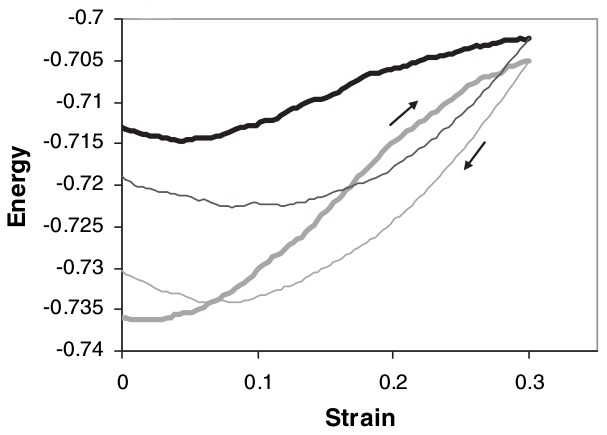
\includegraphics[width=0.7\textwidth]{OscillatoryRejuvenationNK.png} 
\caption{Energy per site as a function of strain in an athermal quasi static deformation of a NK system, by varying $\gamma$ from $0$ to $\gamma_{max} = 0.3$ and back to $0$ again, for samples at two different effective temperatures. The sample at initial lower effective temperature rejuvenates after a semicycle of deformation (gray data), whereas the sample at initial higher temperature overages (black). Note the similarity with what is observed in \autoref{fig:OscillatoryRejuvenationLJ}. From \cite{isner2006generic}. \label{fig:OscillatoryRejuvenationNK}}
\end{figure}

\subsection{Coarse-grained approach to the deformation of amorphous solids}
Considerable effort has also been put into the understanding of the microscopic origins of the macroscopic mechanical properties listed in \autoref{sec:DeformedGlasses}, with special attention to the behavior beyond the elastic limit, which is critical for applications. In particular, recently theoretical work has been carried out so to build a framework comparable to that that is able to describe deformation in crystalline solids. In the case of crystalline solids, plastic deformation can be rationalized by the nucleation, motion and interaction of crystal defects such as dislocations \cite{phillips1999hierarchical, shilkrot2002coupled}. Established models of interactions between dislocations in crystals exist, which can be connected to finer-grained atomistic simulations \cite{bulatov1998connecting}, but this is not yet the case for amorphous solids. An attempt to fill this gap is represented by the shear transformation zone (STZ) theory \cite{langer2006shear}, preceded by other models \cite{argon1979plastic, spaepen1977microscopic}.\\
The STZ theory assumes that the bulk of the material is populated by some number $\Lambda$ of structural fluctuations that are capable to ``transform'' (change their state) as a shear stress $\sigma$ is applied to the sample. In the STZ theory, the density of such fluctuations depends on an ``effective disorder'' parameter $\chi$, and $\chi$ is also dependent on $\sigma$ and the temperature $T$. In turn $\sigma$ can be related to the strain $\gamma$ via a linear proportionality related to the elastic modulus of the material $\mu$.
The above relations constitute a set of coupled equations of the evolution of the applied strain $\gamma$, $\sigma$, $\Lambda$, $\chi$, which can be solved as a function of the time $t$ for a given applied strain profile $\gamma(t)$. In this way, one can thus determine \cite{bouchbinder2013private} the relation existing between the strain and the stress for oscillatory deformation simulations like those performed in \cite{lacks2004energy}, and like those that are presented in the next chapters.

\section{Oscillatory driven suspensions, memory effects}

\subsection{Results on non-brownian suspensions relevant for this work\label{sec:ShearedSuspensions}}

One of the aims of this thesis is to compare the behavior exhibited by oscillatory sheared glasses in simulations like those listed in \autoref{sec:PreviousWorkOnOveragingAndRejuvenation} to that observed in oscillatory deformation experiments of a completely different system: a suspension of dilute non-brownian particles. The idea is to explore the similarities (if any) and differences between the two classes of systems. \\
An example of suspension of dilute non-brownian particles is given by the system studied in \cite{corte2008random}. 
In \cite{corte2008random}, solid beads of polymethylmethacrylate of size $\approx \SI{200}{\micro\metre}$ are immersed in a viscous solution of water and surfactants. The beads and the surrounding medium have the same density (so that the weight of the particles is balanced exactly by buoyancy) and the same index of refraction (so to reduce as much as possible attraction due to Van der Waals forces). The particles are also big enough so that Brownian motion is absent. 
The resulting suspension is sheared repeatedly in an oscillatory way, up to some amplitude $\gamma_{max}$. Upon shearing and in the absence of collisions between them, particles move in such a way that the coordinates $\mathbf{r_{i}}$ of the center of particle $i$ transform according to the affine map:
\begin{align}
	A \mathbf{r} &= \mathbf{r'}\\
	\begin{pmatrix}
		1 & \gamma & 0 \\
		0 & 1 & 0 \\
		0 & 0 & 1 \\
	\end{pmatrix}
	\begin{pmatrix}
		x \\
		y \\
		z
	\end{pmatrix} &=  
	\begin{pmatrix}
		x + \gamma y \\
		y \\
		z
	\end{pmatrix}
	\label{eq:ShearDeformationMatrix}
\end{align} 
where $\gamma$ is a periodic function of time. In that case the motion is clearly reversible and the particles move in orbits which are retraced over and over again.
However, if two particles become in contact in the course of the deformation, they interact irreversibly and do not retrace the trajectory followed before. This behavior can be modeled (see \cite{corte2008random} and \autoref{fig:ShearedSuspensionSetup}) by assuming that particles move according to \autoref{eq:ShearDeformationMatrix} as long as no collisions occur and are displaced in a random way whenever they collide.\\

\begin{figure} 
\centering 
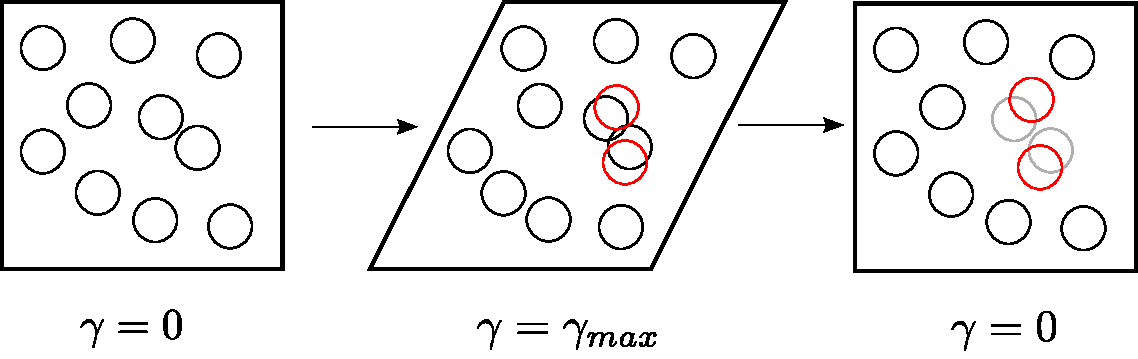
\includegraphics[width=0.8\textwidth]{ActiveParticles.pdf} 
\caption{Schematic of the dynamics of the system in \cite{corte2008random} in the course of a deformation semicycle. The system is affinely shear deformed up to some maximum value $\gamma_{max}$, according to \autoref{eq:ShearDeformationMatrix}. Some of the particles come in contact in the course of such deformation. Those which do are labeled in red and named \emph{active} (see text). Active particles are displaced randomly right after the collision. At the completion of a deformation semicycle, the result is that particles that haven't experienced any collision do get back to the position they started from, whereas the active ones are displaced from their original position (labeled in gray). \label{fig:ShearedSuspensionSetup}}
\end{figure}

If samples are let evolve according to this dynamics and are observed stroboscopically at $\gamma = 0$, one can distinguish two different kinds of particles, by comparing the configurations of the system assumed before and after a deformation cycle: 
\begin{itemize}
	\item some of the particles won't change their position. These are the particles which haven't experienced any collision in the shear oscillation cycle.
	\item the rest of the particles will move, because they have collided in the course of the cycle, and we refer to them as \emph{active}.
\end{itemize}

\subsubsection{Existence of a transition amplitude $\gamma_{c}$}

An interesting transition in behavior is observed if a large number of shear oscillations is performed: 

\begin{itemize}
\item for values of $\gamma_{max}$ below some threshold value $\gamma_{c}$, after some average characteristic number of oscillations $\tau_{-}(\gamma_{max})$, the system reaches a state where \emph{no particle is active}. This is because random collisions bring the system to states such that no particles collide in the course of a shear cycle. Such quiescent states are named \emph{absorbing}.
\item for values of $\gamma_{max}$ above the threshold value $\gamma_{c}$, instead, a fraction $f_{a}$ of the particles is always active, and the systems never seem to reach an absorbing state. Additionally, $f_{a}$ seems to approach an asymptotic value in a characteristic number of oscillations $\tau_{+}(\gamma_{max})$, and thus the system reaches a \emph{stationary} state (at least by judging from the value of $f_{a}$). The $f_{a}$ measured in a stationary state depends on $\gamma_{max}$ (see \autoref{eq:ActiveFractionVsGammaMax}).
\end{itemize}

Experimental data on $f_{a}$ in a 3D system and in simulations of a 2D system \cite{corte2008random} do yield the form
\begin{equation}
	f_{a}(\gamma_{max}) = 
	\left\{ 
	\begin{array}{rl}
		0 & \text{if } \gamma_{max} < \gamma_{c}  \\
		(\gamma_{max} - \gamma_{c})^{\beta} & \text{if } \gamma_{max} \geq \gamma_{c}
	\end{array}
	\right.
	\label{eq:ActiveFractionVsGammaMax}
\end{equation}

This behavior, observed in the 2D simulations in \cite{corte2008random}, is displayed in \autoref{fig:ActiveFractionVsGammaMax}.

\begin{figure} 
\centering 
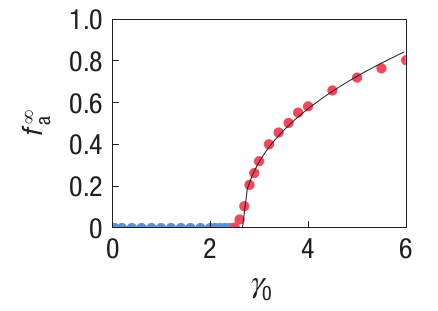
\includegraphics[width=0.45\textwidth]{ActiveFractionVsGammaMax.png} 
\caption{Fraction of active particles (see text) observed after a large number of oscillation cycles (larger than some characteristic $\tau$) as a function of the oscillation amplitude (here indicated with $\gamma_{0}$) in a model of a sheared suspension (see text). A transition at some value $\gamma_{c}$ is observed. From \cite{corte2008random}. \label{fig:ActiveFractionVsGammaMax}}
\end{figure}

In addition, the values of the characteristic numbers of oscillations $\tau_{\pm}(\gamma_{max})$ seem to follow, in the same cases, the dependence
\begin{equation}
	\tau_{\pm}(\gamma_{max}) = |\gamma_{max} - \gamma_{c}|^{-\nu_{\pm}}
	\label{eq:TauVsGammaMax}
\end{equation}
signalling a divergence of the number of oscillations $\tau_{-}$ needed to reach an absorbing state below $\gamma_{c}$ and $\tau_{+}$ needed to reach a stationary state above $\gamma_{c}$.
This behavior, observed in the 2D simulation in \cite{corte2008random}, is displayed in \autoref{fig:TauVsGammaMax}.
The values of the exponents $\beta$ and $\tau_{\pm}$ can be obtained theoretically \cite{menon2009universality} in 2D and 3D, and have been suggested to be those that pertain to the universality class of conserved directed percolation \cite{hinrichsen2000nonequilibrium}.

\begin{figure} 
\centering 
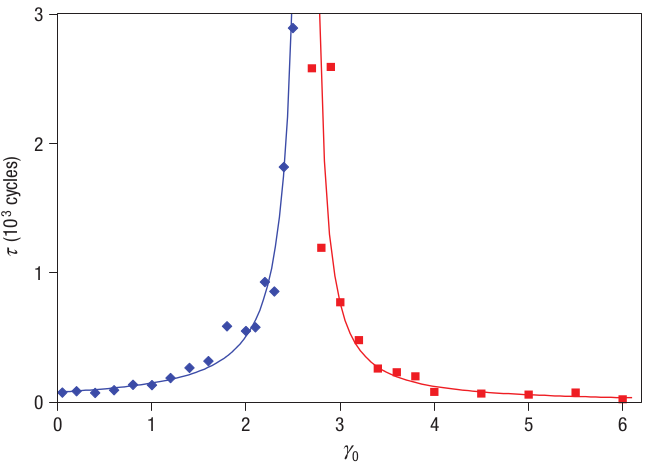
\includegraphics[width=0.8\textwidth]{TauVsGammaMax.png} 
\caption{Characteristic number of shear oscillations $\tau_{-}$ (blue) and $\tau_{+}$ needed to the the number of active particles in the model colloidal suspension in \cite{corte2008random} to approach a constant value as a function of the oscillation amplitude. At some value $\gamma_{c}$ $\tau$ is seen to diverge. From \cite{corte2008random}. \label{fig:TauVsGammaMax}}
\end{figure}

\subsubsection{Memory effects}
From what has been said above, if an experimenter shear deforms a suspension of the kind described in \autoref{sec:ShearedSuspensions} in a cyclic way up to some value $\gamma_{1} < \gamma_{c}$, the system eventually reaches a final absorbing state which it can't leave. 
It turns out that if such a final state is handed to some other experimenter, she can determine the amplitude $\gamma_{1}$ from simple measurements on the sample.
To understand this, one can note that as the sample is in an absorbing state for oscillations of amplitude $\gamma_{1}$, any shear deformation cycle of amplitude $\gamma_{r} < \gamma_{1}$ will leave the sample unaltered. This is because if no collision occurs during a shear deformation cycle of amplitude $\gamma_{1}$ (which is the necessary condition for the state to be absorbing for that amplitude) no collision can occur for any deformation of a smaller amplitude\footnote{This fact is called ``ordering of reversible states'' in \cite{keim2011generic}.}. As soon as $\gamma_{r}$ is raised above $\gamma_{c}$, however, collisions \emph{can occur}, and the configuration of the system can be modified by a single cycle of shear deformation.
All of the above can be exploited so to \emph{read} the value of $\gamma_{1}$: one simply needs to apply cyclic shear deformation to the samples starting from an amplitude $\gamma_{r} = 0$, perform wider and wider oscillations and measure the fraction of active particles. Initially the sample will be unaltered (with zero active particles), but for some value $\gamma^{*} \geq \gamma_{c}$ the system will be perturbed (with nonzero active particles). This is shown in \autoref{fig:SuspensionSingleMemory} in the curve which represents the fraction of active particles in samples which have undergone $\approx 55000$ shear oscillations at $\gamma_{1} = 3$. The value of $\gamma^{*}$ is an \emph{upper bound} for $\gamma_{1}$, and can be considered a good approximation of it.\\
From all of this one can conclude that if a first experimenter \emph{trains} a sample by shearing it cyclically, a second one can \emph{read} the value of the amplitude of the training oscillations in the way described above. The samples are thus able to store a \emph{memory} of their mechanical history.

The fact that the approach to an absorbing state is exponential (described by $\tau_{-}$) has an important consequence. 
Let's consider a collection of samples, on which an experimenter performs a number $\tau < \tau_{-}$ of oscillations of amplitude $\gamma_{1}$. The training of the samples will be, so to say, ``incomplete'': this means that some of the samples will reach an absorbing state for $\gamma_{1}$, and others will not. A ``reading experiment'' will be able to reveal the value of $\gamma_{1}$, by measuring a ``kink'' in the average number of active particles $f_{a}$ as a function of $\gamma_{r}$, due to the signal from the samples that have reached an absorbing state for $\gamma_{1}$. An example of such a kink is evident in the curves in  \autoref{fig:SuspensionSingleMemory} relative to incomplete trainings (those labeled with a number of oscillations $\leq 1000$).
If such ``partially trained'' collection of samples is now cyclically shear deformed up to $\gamma_{2} < \gamma_{1}$, after some cycles some of the samples will become absorbing for $\gamma_{2}$. The collection of samples will thus be divided in three sets at that point:
\begin{enumerate*}[label=\itshape\alph*\upshape)]
	\item absorbing states for $\gamma_{2}$, but which are not absorbing for $\gamma_{1}$;
	\item absorbing states for $\gamma_{1}$ (absorbing \emph{also} for $\gamma_{2}$);
	\item states that are not absorbing neither for $\gamma_{2}$ nor for $\gamma_{1}$.
\end{enumerate*}
A ``reading experiment'' measuring $f_{a}$ as a function of $\gamma_{r}$ will thus show two kinks in correspondence of $\gamma_{1}$ and $\gamma_{2}$. This procedure can be generalized to more training amplitudes $\gamma_{1} > \gamma_{2} > \ldots$, and proves that these kinds of systems are able to store \emph{multiple} memories.\\
In \cite{keim2011generic}, multiple memories are encoded in samples by training them alternating a small number oscillations of different amplitudes, so that the strain $\gamma$ of the sample varies in cycles $0 \rightarrow \gamma_{1} \rightarrow 0 \rightarrow  -\gamma_{1} \rightarrow 0 \rightarrow \gamma_{2} \rightarrow 0 \rightarrow  -\gamma_{2} \rightarrow 0$. The result of a reading operation on samples treated this way is shown in \autoref{fig:SuspensionDoubleMemory}.
Moreover, such multiple memories are shown to be \emph{transient}, that is they're erased if the training is long enough. This is because oscillations of amplitude $\gamma_{1}$ make the system evolve to absorbing states for this amplitude, and the amplitudes $\gamma_{i} < \gamma_{1}$ are unable, by construction, to destabilize such absorbing states. The effect of a long series of alternated oscillations of multiple amplitudes $\gamma_{1} > \gamma_{2} > \ldots$ is thus to produce a set of absorbing states for the largest amplitude $\gamma_{1}$ only, that retain no memory of the smaller amplitudes. This is evident in \autoref{fig:SuspensionDoubleMemory} in the reading of samples trained with $\approx 30000$ shear oscillations.

\begin{figure} 
	\centering
	\begin{subfigure}[b]{0.45\textwidth}
		\centering
		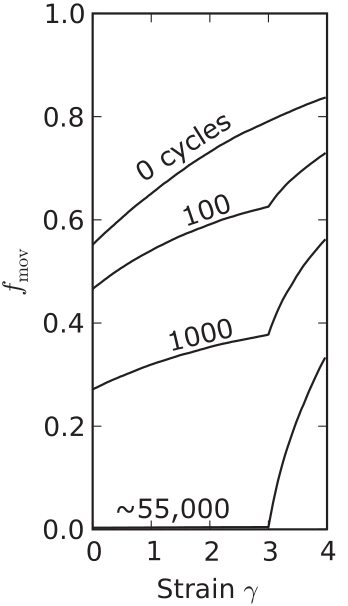
\includegraphics[scale = 0.4]{SuspensionSingleMemory.png}
		\caption{\label{fig:SuspensionSingleMemory}}
	\end{subfigure}
	\centering
	\begin{subfigure}[b]{0.45\textwidth}
		\centering
		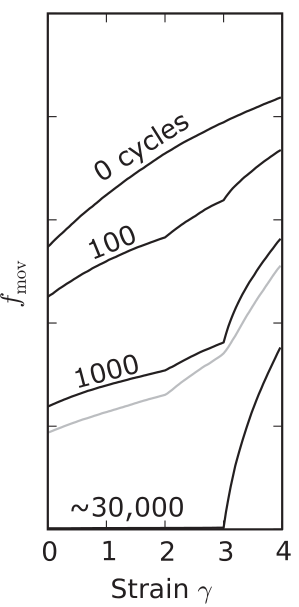
\includegraphics[scale = 0.4]{SuspensionDoubleMemory.png}
		\caption{\label{fig:SuspensionDoubleMemory}}
	\end{subfigure} 
\caption{(\subref{fig:SuspensionSingleMemory}) Number of active particles as a function of the reading amplitude (here labeled with $\gamma$) for a model of suspension subjected to a series of oscillations of amplitude $\gamma_{1}=3$ and of different durations (specified next to the curves). The reading reveals the presence of memory of the initial training, and for a large number of oscillations no active particles are observed in the reading below $\gamma_{1}$. (\subref{fig:SuspensionDoubleMemory}) In black: number of active particles read from samples trained by a series of oscillations alternating two different amplitudes $\gamma_{1}=3, \gamma_{2}=2$. The trace of a double memory of the training is evident but for the longest training. The multiple memory is transient. In gray: number of active particles subjected to a very long training alternating two oscillations amplitudes and adding noise in the dynamics. The multiple memory is still present, and is thus stabilized by the noise. From \cite{keim2011generic}. \label{fig:SuspensionMemory}}
\end{figure}

The erasure of the memory left by training at amplitudes smaller than $\gamma_{1}$ can be avoided via the addition of a simple ingredient: noise. In \cite{keim2011generic}, authors show that by adding a random perturbation to the trajectories, so that they ``wiggle'' around the path prescribed by \autoref{eq:ShearDeformationMatrix}, multiple memories can be stabilized. The consequence of the addition of such noise is that cycles of smaller amplitudes are able to destabilize absorbing states for larger amplitudes, making multiple memories \emph{persistent} under the application of an indefinitely large number of training cycles. The result of a reading experiment on a system subjected to a large number of alternating cycles with two amplitudes $\gamma_{1}$ and $\gamma_{2}$ in the presence of noise is shown in \autoref{fig:SuspensionDoubleMemory}, in gray.

\section{Summary}

In the previous paragraphs we have briefly outlined the main features of metallic glasses, considering their mechanical properties and their formation. Metallic glasses are a subclass of materials in the larger family of glasses, and thus their properties can be studied (at least qualitatively) with theoretical and simulation techniques developed to describe glassy systems. \\
Simulations of oscillatory shear deformation performed in the past show that glassy systems rearrange so to change their potential energy under applied strain \cite{lacks2004energy, utz2000atomistic}. In particular, \emph{rejuvenation} and \emph{overaging} are observed by analyzing a \emph{single} cycle of shear deformation in Lennard-Jones models.
It is however unclear what is the potential energy behavior of samples subject to a \emph{large} number of deformation cycles, like in fatigue experiments in which a cyclic load is applied on a sample. This issue is explored in the chapters that follow.\\
It is interesting to ask also how particles composing a system deformed in the way described above \emph{move} in the course of deformation. This kind of dynamics has been investigated in the case of shear deformed dilute noncolloidal suspensions \cite{corte2008random}, which show a \emph{non-equilibrium transition} in the motion of the suspended particles as a function of the oscillatory deformation amplitude. In the following chapters (among the rest) we will explore similarities between the phenomenology observed in noncolloidal suspensions and particle models of glassy systems.
